% mnras_template.tex
%
% LaTeX template for creating an MNRAS paper
%
% v3.0 released 14 May 2015
% (version numbers match those of mnras.cls)
%
% Copyright (C) Royal Astronomical Society 2015
% Authors:
% Keith T. Smith (Royal Astronomical Society)

% Change log
%
% v3.0 May 2015
%    Renamed to match the new package name
%    Version number matches mnras.cls
%    A few minor tweaks to wording
% v1.0 September 2013
%    Beta testing only - never publicly released
%    First version: a simple (ish) template for creating an MNRAS paper

%%%%%%%%%%%%%%%%%%%%%%%%%%%%%%%%%%%%%%%%%%%%%%%%%%
% Basic setup. Most papers should leave these options alone.
\documentclass[fleqn,usenatbib]{mnras}

% MNRAS is set in Times font. If you don't have this installed (most LaTeX
% installations will be fine) or prefer the old Computer Modern fonts, comment
% out the following line
\usepackage{newtxtext,newtxmath}
% Depending on your LaTeX fonts installation, you might get better results with one of these:
%\usepackage{mathptmx}
%\usepackage{txfonts}

% Use vector fonts, so it zooms properly in on-screen viewing software
% Don't change these lines unless you know what you are doing
\usepackage[T1]{fontenc}
\usepackage{ae,aecompl}


%%%%% AUTHORS - PLACE YOUR OWN PACKAGES HERE %%%%%

% Only include extra packages if you really need them. Common packages are:
\usepackage{graphicx} % Including figure files
\usepackage{amsmath} % Advanced maths commands
\usepackage{amssymb} % Extra maths symbols

%%%%%%%%%%%%%%%%%%%%%%%%%%%%%%%%%%%%%%%%%%%%%%%%%%

%%%%% AUTHORS - PLACE YOUR OWN COMMANDS HERE %%%%%

% Please keep new commands to a minimum, and use \newcommand not \def to avoid
% overwriting existing commands. Example:
%\newcommand{\pcm}{\,cm$^{-2}$} % per cm-squared

% Use bold font for vectors
\let\vec\mathbf

%%%%%%%%%%%%%%%%%%%%%%%%%%%%%%%%%%%%%%%%%%%%%%%%%%

%%%%%%%%%%%%%%%%%%% TITLE PAGE %%%%%%%%%%%%%%%%%%%

% Title of the paper, and the short title which is used in the headers.
% Keep the title short and informative.
\title[Hybrid multigrain]{Hybrid multigrain: A smoothed particle hydrodynamics
algorithm for small and large dust grains}

% The list of authors, and the short list which is used in the headers.
% If you need two or more lines of authors, add an extra line using \newauthor
\author[Mentiplay, Price, Laibe, \& Pinte]{%
   \parbox{\textwidth}{%
      Daniel Mentiplay$^{1}$\thanks{daniel.mentiplay@monash.edu},
      Daniel J. Price$^{1}$,
      Guillaume Laibe$^{2}$,
      Christophe Pinte$^{1,3}$}\\
   $^{1}$Monash Centre for Astrophysics (MoCA) and School of Physics and
   Astronomy, Monash University, Clayton Vic 3800, Australia \\
   $^{2}$Lyon, France \\
   $^{3}$Univ. Grenoble Alpes, CNRS, IPAG, F-38000 Grenoble, France}

% These dates will be filled out by the publisher
\date{Accepted XXX. Received YYY; in original form ZZZ}

% Enter the current year, for the copyright statements etc.
\pubyear{2020}

% Don't change these lines
\begin{document}
\label{firstpage}
\pagerange{\pageref{firstpage}--\pageref{lastpage}}
\maketitle

% Abstract of the paper
\begin{abstract}
\end{abstract}

% Select between one and six entries from the list of approved keywords.
% Don't make up new ones.
\begin{keywords}
keyword1 -- keyword2 -- keyword3
\end{keywords}

%%%%%%%%%%%%%%%%%%%%%%%%%%%%%%%%%%%%%%%%%%%%%%%%%%

%%%%%%%%%%%%%%%%% BODY OF PAPER %%%%%%%%%%%%%%%%%%

\section{Introduction}

\section{Methods}

The equations of conservation of momentum for a multiple species dust and gas
mixture are given by
%
\begin{align}
   \rho_g \frac{d \vec{v}_g}{dt} &= - \nabla P + \sum_i K_i \left(\vec{v}_{d_i}
                                    - \vec{v}_{g}\right), \\
   \rho_{d_i} \frac{d \vec{v}_{d_i}}{dt} &= - K_i \left(\vec{v}_{d_i}
                                                       - \vec{v}_{g}\right),
\end{align}
%



\section{Numerical tests}

\subsection{Dustybox}

No back-reaction, low dust-to-gas ratio:

\begin{itemize}

   \item dustybox: Epstein sub-sonic drag (linear regime) one grain size
   \item dustybox: Epstein sub-sonic drag (linear regime) multiple grains
   \item dustybox: Stokes regime
   \item sub- and super-sonic
\end{itemize}

\begin{figure*}
    \begin{center}
      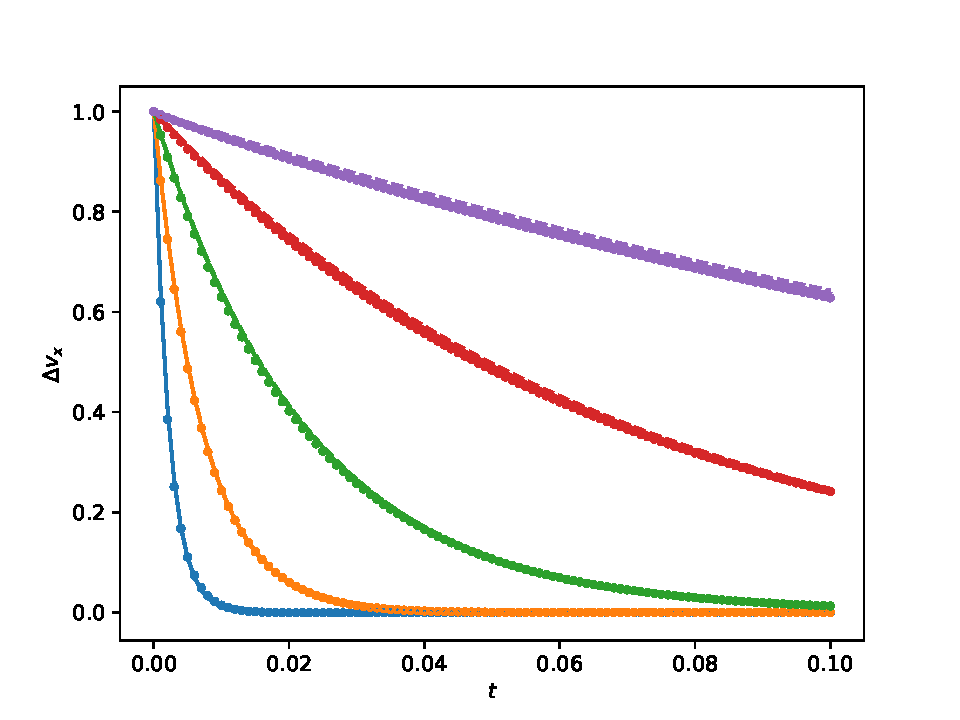
\includegraphics[width=\columnwidth]{figs/delta_vx_Epstein-f=0_01.pdf}
      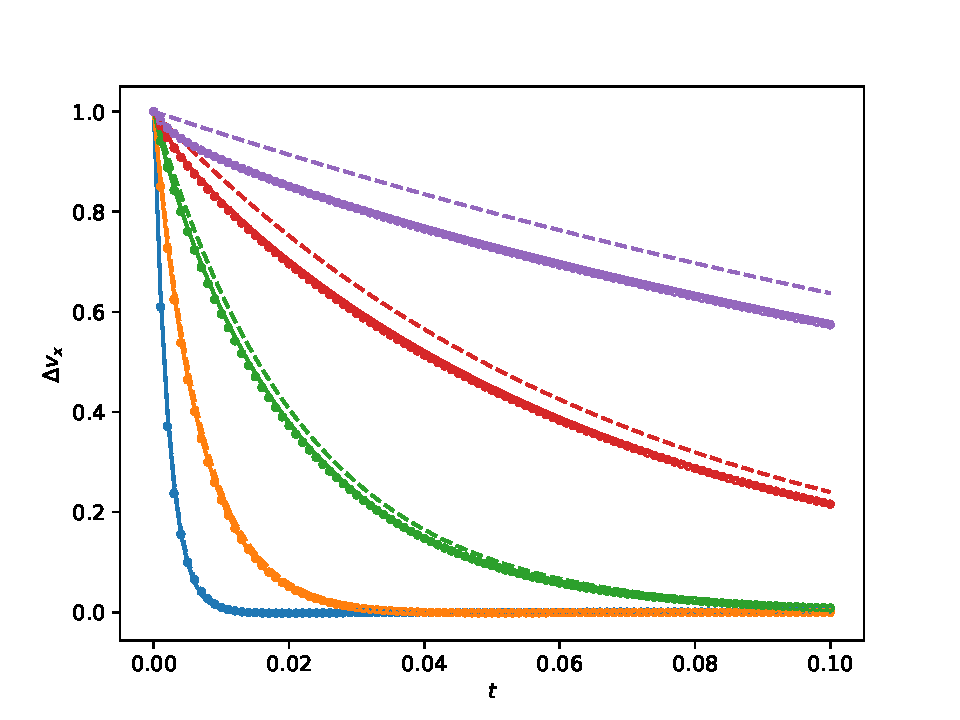
\includegraphics[width=\columnwidth]{figs/delta_vx_Epstein-f=0_1.pdf}
      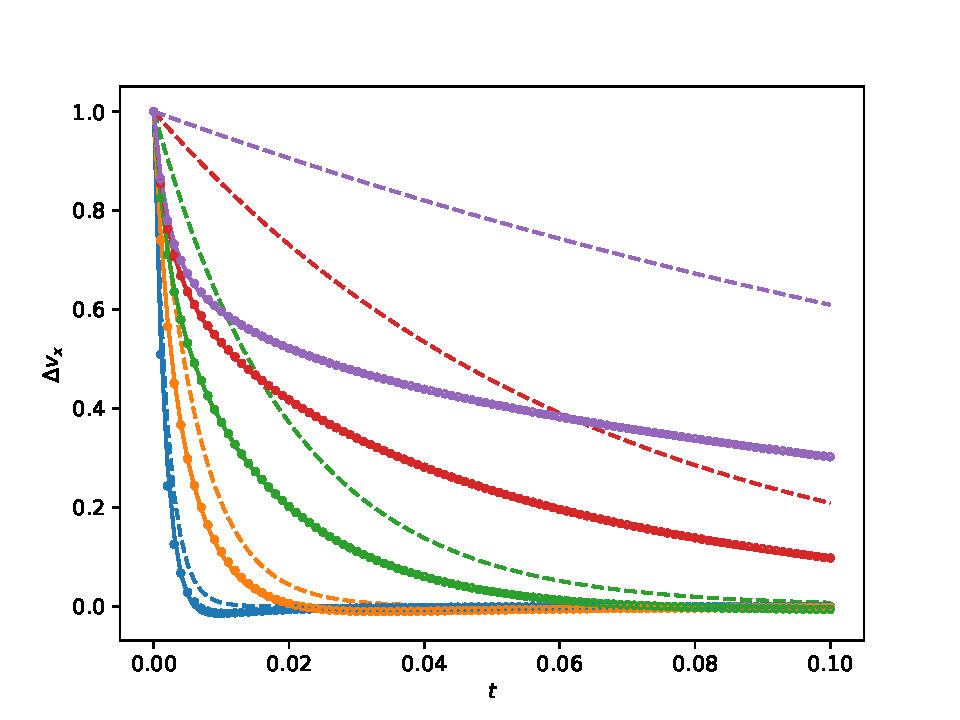
\includegraphics[width=\columnwidth]{figs/delta_vx_Epstein-f=1_0.pdf}
      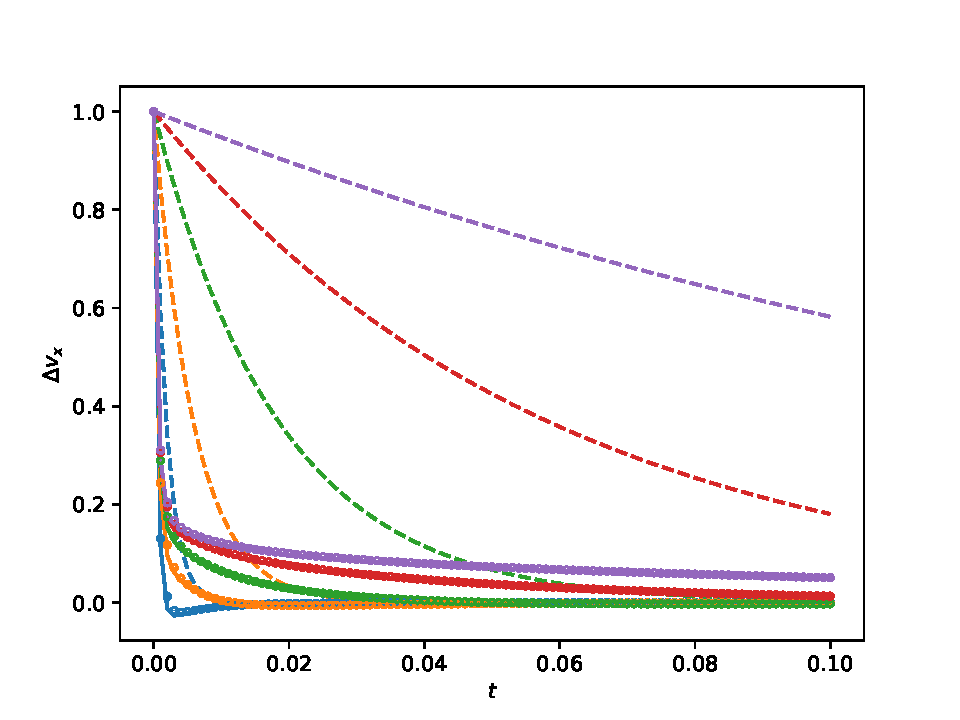
\includegraphics[width=\columnwidth]{figs/delta_vx_Epstein-f=10_0.pdf}
      \caption{Dustybox: (a) dust-to-gas ratio = 0.01, (b) dust-to-gas ratio
      = 0.1, (c) dust-to-gas ratio = 1.0, (d) dust-to-gas ratio = 10.0}
    \end{center}
\end{figure*}

With back-reaction.

\subsection{Dustywave}

Same collection of tests as dustybox.

\subsection{Dustyshock}
See Benitez-Llambay paper.

\section{Application}

\subsection{Circumbinary disc}

Do a comparison between multiple single grain calculations vs one multigrain
calculation focussing on dust trapping in a circumbinary disc. The figure would
show a phase difference between the dust (or gas) distribution comparing the
single-grain vs multigrain calculation.

\section{Discussion}

\section{Conclusions}

\section*{Acknowledgements}


%%%%%%%%%%%%%%%%%%%%%%%%%%%%%%%%%%%%%%%%%%%%%%%%%%

%%%%%%%%%%%%%%%%%%%% REFERENCES %%%%%%%%%%%%%%%%%%

% The best way to enter references is to use BibTeX:

\bibliographystyle{mnras}
% \bibliography{references}


%%%%%%%%%%%%%%%%%%%%%%%%%%%%%%%%%%%%%%%%%%%%%%%%%%

%%%%%%%%%%%%%%%%% APPENDICES %%%%%%%%%%%%%%%%%%%%%

% \appendix

% \section{Some extra material}


%%%%%%%%%%%%%%%%%%%%%%%%%%%%%%%%%%%%%%%%%%%%%%%%%%


% Don't change these lines
\bsp % typesetting comment
\label{lastpage}
\end{document}
% End of mnras_template.tex
